\section{Evaluation}
\label{sec:evaluation}

% \subsection{Research Questions}

We investigate key research questions to validate the effectiveness and efficiency of \sys:

\begin{itemize}
\item \textbf{RQ1}: Can \sys effectively configure existing schedulers?
\item \textbf{RQ2}: Can \sys generate new schedulers for specific workloads?
\item \textbf{RQ3}: What is the cost and efficiency of \sys's scheduler generation?
\item \textbf{RQ4}: How much can \agent continue to improve performance after initial generation?
% \item \textbf{RQ5}: How effectively can \sys understand workloads?
\end{itemize}

\subsection{Experimental Setup}

We evaluate \sys on two machines, machine 1 is an 86-core, 172 threads Intel Xeon 6787P with 758GB RAM, NVMe SSDs, 10Gbps network, with 2x 256 GB CXL (Compute Express Link) memory device, 3 numa node, running Linux 6.14 with sched\_ext. Machine 2 is an 8-core, 8 threads Intel Core Ultra 7 258V with 30GB RAM, NVMe SSDs, 1 NUMA node, running Linux 6.13 with sched\_ext. We test Claude Code (Opus 4) as AI agents to validate framework generality. For each case, we test 3 times and get the average results.

\subsection{Performance Impact of AI-Driven Optimization}

Figure~\ref{fig:performance-comparison} shows performance improvements across three stages: baseline EEVDF, LLM-configured schedulers, and Iteration-improved configurations. We also compare with basic RL algorithms that have been proposed for scheduler optimization~\cite{corbet2025ml}.

% For schbench, the LLM achieves 50\% lower p99 latency and 30\% higher throughput by selecting scx\_layered. 

The Linux kernel build benchmark compile the kernel 6.14 with tinyconfig and ``make -j 172'' on machine 1. The workload shows 1.63x speedup from 13.57s to 8.31s using scx\_rusty as the first attemp. After 3 iteration of observe-optimization process, the \agent selects the scx\_layered scheduler and adds 16\% additional gain beyond LLM configuration, with total improvements of 1.79x over baseline EEVDF. In contrast, basic RL approaches show no improvement in our tests, likely because they require hardware-specific retraining, which is costly and time-consuming. 

\begin{figure}[h]
\centering
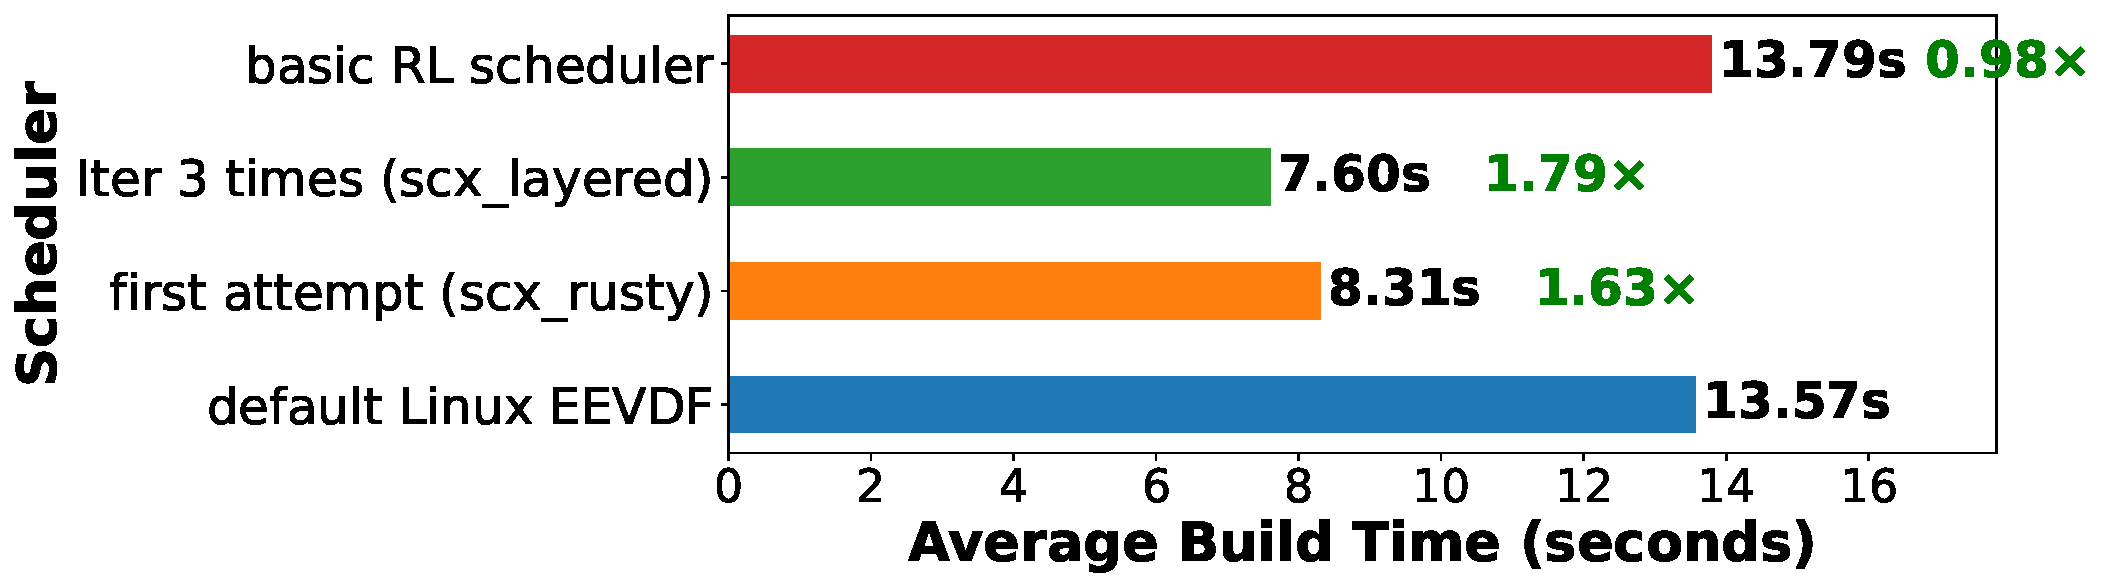
\includegraphics[width=0.9\columnwidth]{sections/Linux_build_benchmark_results.pdf}
\caption{Performance comparison of scheduler configurations.}
\label{fig:performance-comparison}
\end{figure}

\subsection{Scheduler Synthesis for Batch Workloads}

Figure~\ref{fig:batch-performance} demonstrates AI-generated scheduler performance on batch processing workloads. We selected 8 diverse workloads from real-world scenarios including file compression, video transcoding, software testing, and data analytics tasks, each configured with 40 parallel tasks (39 short tasks completing in seconds, 1 long task taking significantly longer) to create severe load imbalance typical of long-tail distributions. We execute tasks in parallel and calculate performance improvements for end to end latency in machine 2. We observed the agent can consistently identifies the workload pattens, successfully identify the workload process, implement LJF scheduling and improve the performance for average 20\% reduction in end to end processing time.

Classification cost averages \$0.15 per analysis based on Claude Opus pricing on Aug 2025. We also observed the Agent based on Claude Opus (A bigger and more powerful model for claude code) can successfuly classify all the 8 workloads, while a smaller model Claude sonnet cannot. Beyond performance improvements, our framework achieves cost reductions through systematic optimizations. average Generation time drops from 33 minutes to 2.5 minutes (13x reduction) for one iteration. Monetary cost also falls from \$6.00 to \$0.45.

\begin{figure}[h]
\centering
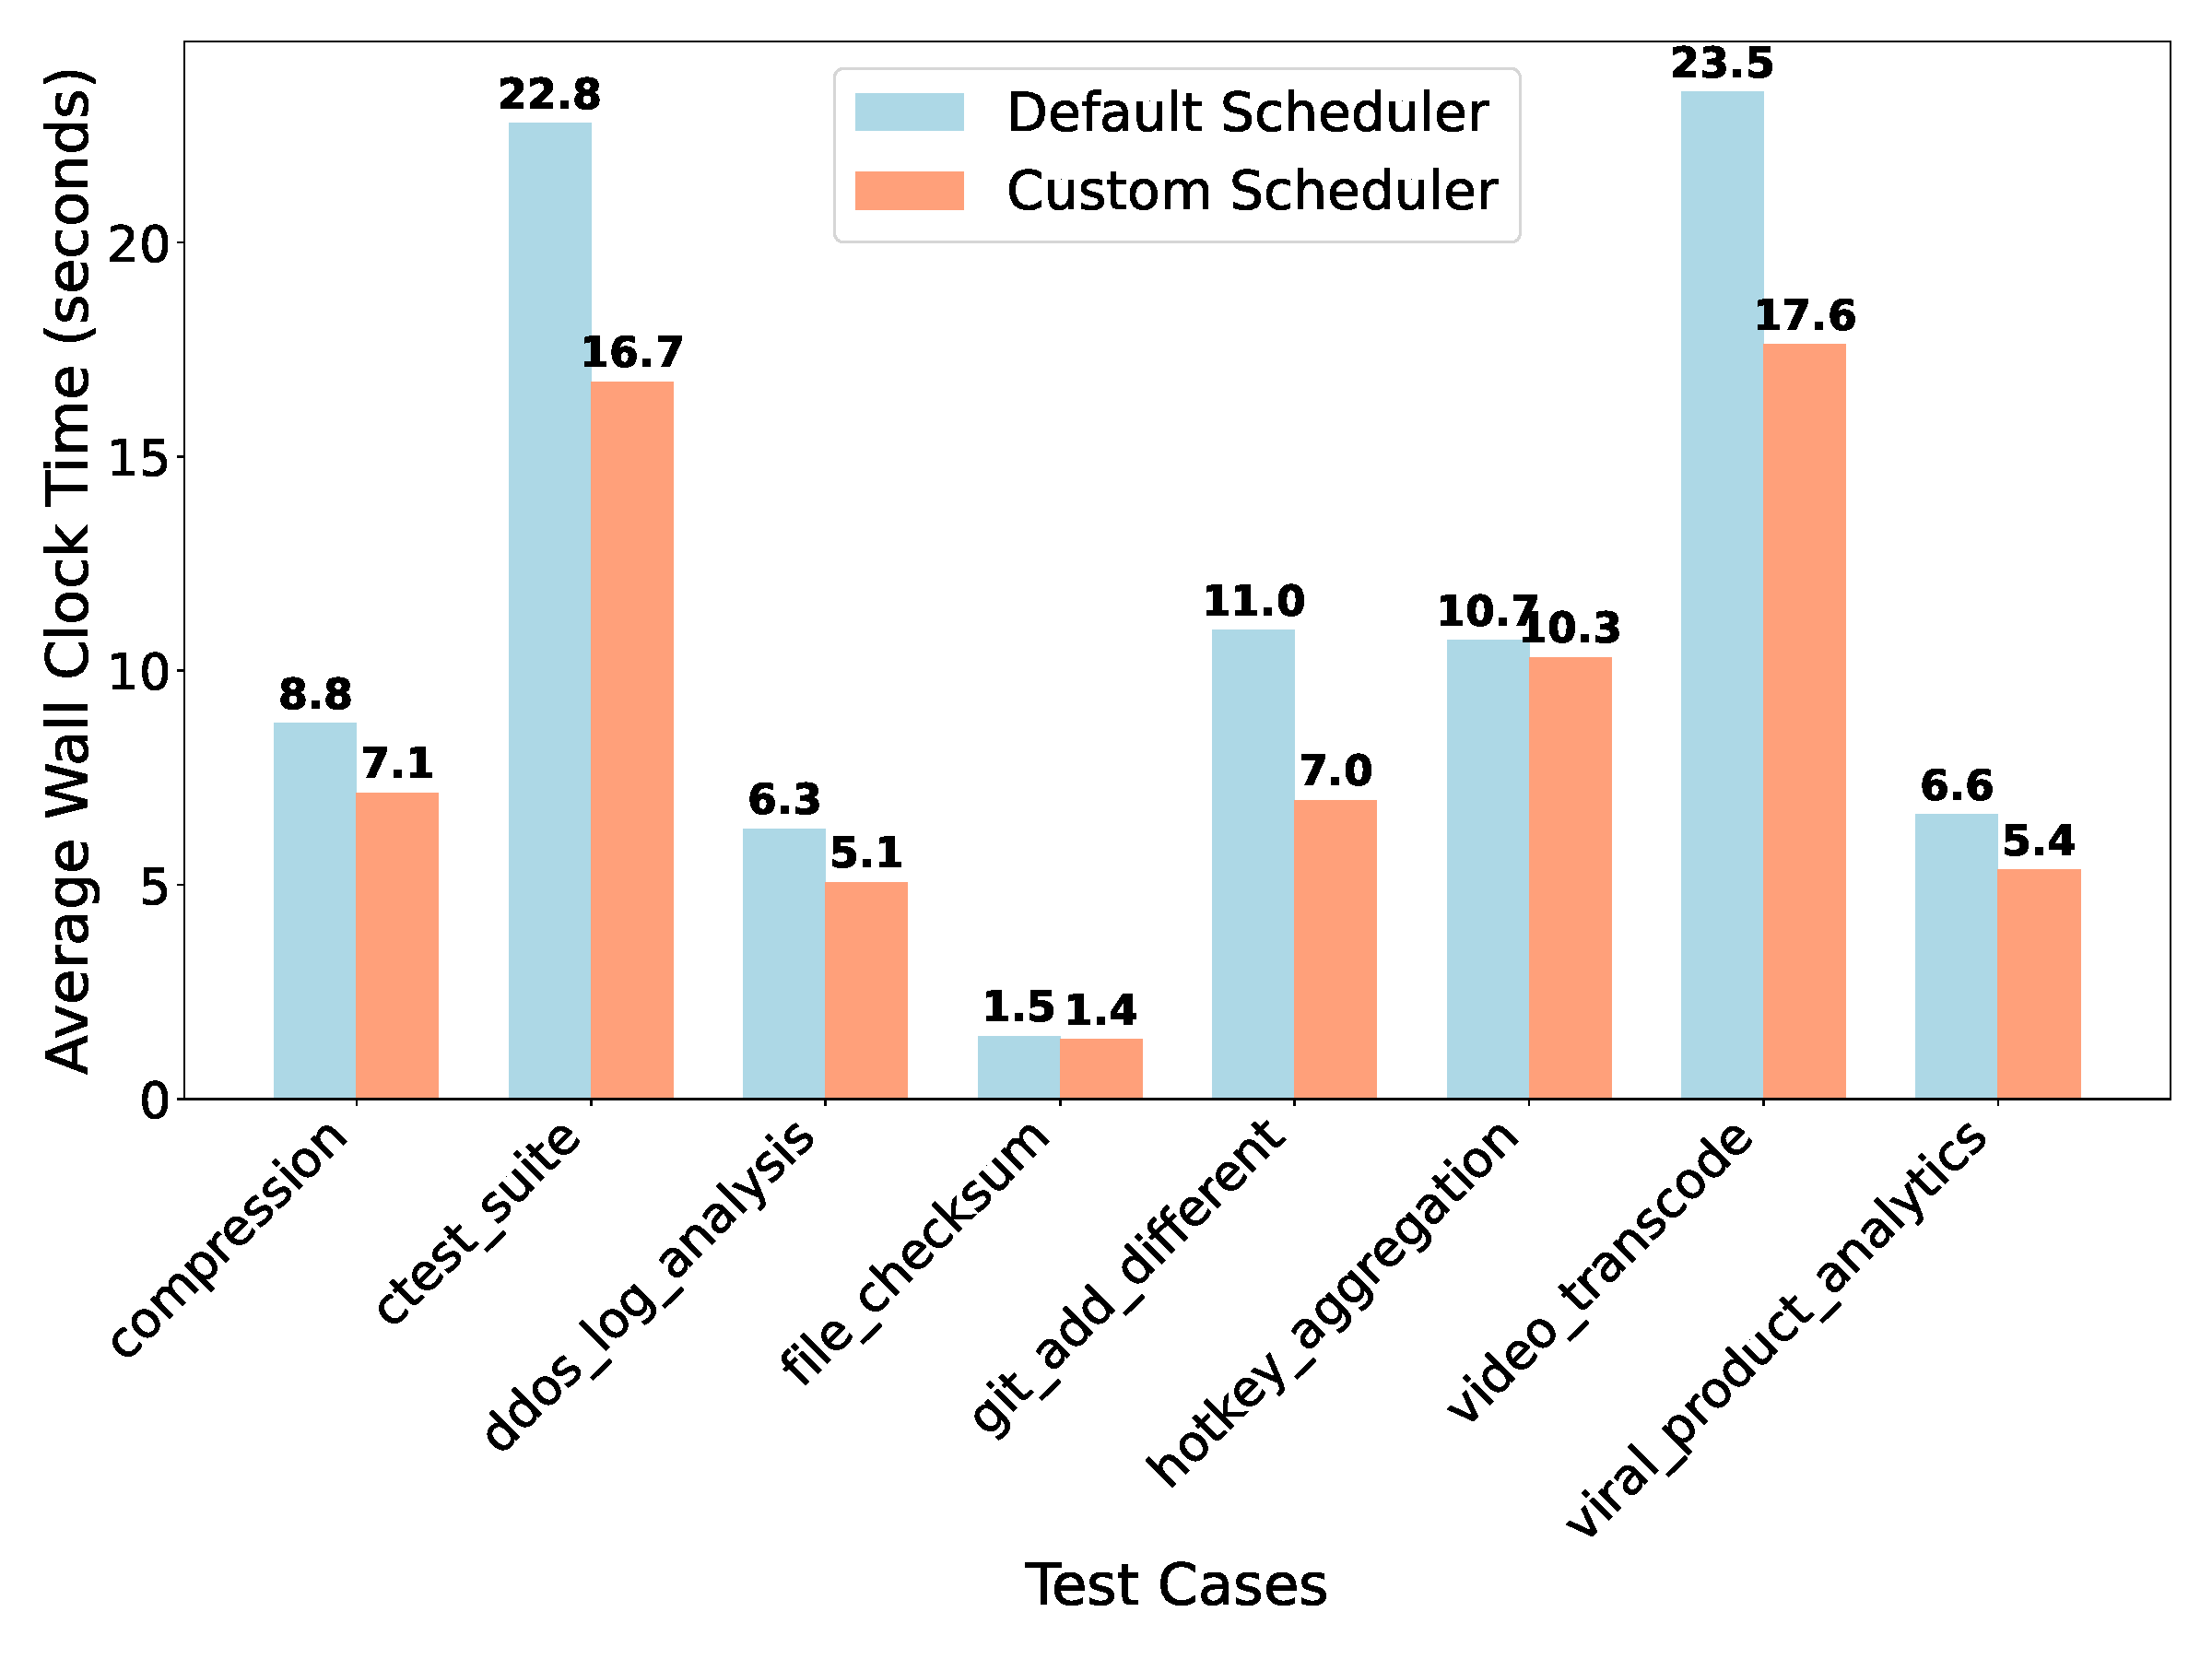
\includegraphics[width=0.9\columnwidth]{sections/scheduler_performance_comparison.pdf}
\caption{AI-generated scheduler performance on batch workloads.}
\label{fig:batch-performance}
\end{figure}


